\documentclass[a5paper,headsepline,titlepage,12pt,nnormalheadings,DIVcalc,twoside]{scrbook}
\usepackage[a5paper,backref]{hyperref}
%\usepackage{palatino}
\usepackage{graphicx}
\usepackage{wrapfig}
\usepackage[bahasa]{babel}
\usepackage{fancyhdr}
\usepackage{pst-text}
\usepackage{pst-grad}

%\setlength{\voffset}{0.5in}
%\setlength{\oddsidemargin}{28pt}
%\setlength{\evensidemargin}{0pt}
\renewcommand{\footrulewidth}{0.5pt}
\lhead[\fancyplain{}{\thepage}]%
      {\fancyplain{}{\rightmark}}
\rhead[\fancyplain{}{\leftmark}]%
      {\fancyplain{}{\thepage}}
\pagestyle{fancy}
\lfoot[\emph{Misa peringatan 1000 hari \namaalm}]{}
\rfoot[]{\emph{Misa peringatan 1000 hari \namaalm}}
\cfoot{}

\makeatletter
\newcommand{\judul}[1]{%
  {\parindent \z@ \centering 
    \interlinepenalty\@M \Large \bfseries #1\par\nobreak \vskip 20\p@ }}
\newcommand{\subjudul}[1]{%
  {\parindent \z@ 
    \interlinepenalty\@M \bfseries #1\par\nobreak \vskip 10\p@ }}
\newcommand{\lagu}[1]{%
  {\parindent \z@ 
    \interlinepenalty\@M \slshape \mdseries \Large \textit{#1}\par\nobreak \vskip 10\p@ }}
\newcommand{\keterangan}[1]{%
  {\parindent \z@  \slshape 
    \interlinepenalty\@M \textsl{#1}\par\nobreak  \vskip 5\p@}}

\renewenvironment{description}
               {\list{}{\labelwidth\z@ \itemindent-\leftmargin
                        \let\makelabel\descriptionlabel}}
               {\endlist}
\renewcommand*\descriptionlabel[1]{\hspace\labelsep 
                                \normalfont\bfseries #1 }


\makeatother

\newcommand{\BU}[1]{\begin{itemize} \item[U:] #1 \end{itemize}}
\newcommand{\BI}[1]{\begin{itemize} \item[I:] #1 \end{itemize}}
\newcommand{\BIU}[1]{\begin{itemize} \item[I+U:] #1 \end{itemize}}
\newcommand{\BP}[1]{\begin{itemize} \item[P:] #1 \end{itemize}}
\newcommand{\inputlagu}[1]{\begin{textit} \input{#1} \end{textit}}
\newcommand{\namaalm}{Bapak Titus Budi Susatyo}
\newcommand{\namaromo}{Heribertus Suprihadi Pr.}

\title{Misa Peringatan 1000 Hari}
\author{\namaalm\\
(12 Februari 1961 - 04 Maret 2007)}
\date{oleh \\ Rm \namaromo\\26 November 2009}
%\hyphenation{sa-u-da-ra-ku}
\hyphenation{ke-ri-ngat}
\hyphenation{je-ri-tan}
\hyphenation{hu-bung-an}
\hyphenation{me-nya-dari}
\hyphenation{Eng-kau}
\hyphenation{ke-sa-lah-an}
\hyphenation{ba-gai-ma-na}
\hyphenation{Tu-han}
\hyphenation{di-per-ca-ya-kan}
\hyphenation{men-ja-uh-kan}
\hyphenation{bu-kan-lah}
\hyphenation{per-sa-tu-kan-lah}
\hyphenation{ma-khluk}
\hyphenation{Sem-buh-kan-lah}
\hyphenation{ja-lan}
\hyphenation{mem-bu-tuh-kan}
\hyphenation{be-ri-kan-lah}
\hyphenation{me-ra-sa-kan}
\hyphenation{te-man-ilah}
\hyphenation{mem-bi-ngung-kan}
\hyphenation{di-ka-gum-i}
\hyphenation{ta-ngis-an-Mu}
\hyphenation{mi-lik-ilah}


\begin{document}
%\maketitle
\thispagestyle{empty}
\newsavebox\IBox
\sbox\IBox{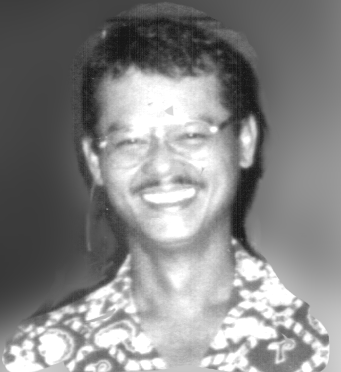
\includegraphics[scale=0.25]{titus.png}}
% set up the picture environment
\psset{unit=1in}
\begin{pspicture}(4in,5in)
% set up the fonts we use
\DeclareFixedFont{\PT}{T1}{ppl}{b}{it}{0.5in}
\DeclareFixedFont{\PTsmall}{T1}{ppl}{b}{it}{0.4in}
\DeclareFixedFont{\PTsmallest}{T1}{ppl}{b}{it}{0.2in}
\DeclareFixedFont{\PTtext}{T1}{ppl}{b}{it}{11pt}
\DeclareFixedFont{\Logo}{T1}{pbk}{m}{n}{0.3in}
% place the front cover picture
\rput[cb](2.3,1.5){\usebox\IBox}
% put the text on the front cover
\rput[cb](2.3,4.5){\PTsmall {EKARISTI}}
\rput[cb](2.3,4.1){\PTsmall {PERINGATAN 1000 HARI}}
\rput[cb](2.3,3.0){\PTsmall {\namaalm}}
\rput[cb](2.3,2.6){\PTsmallest(12 Februari 1961 - 04 Maret 2007)}
\rput[cb](2.3,0.4){\PTsmallest {oleh}} 
\rput[cb](2.3,0){\PTsmallest {Rm \namaromo}}
\rput[cb](2.3,-0.4){\PTsmallest {26 November 2009}}

%\rput[cb](3,-1){\PTsmallest {\namagereja}} 

\end{pspicture}

\newpage
\thispagestyle{empty}
{~}
\newpage

\section*{RITUS PEMBUKA} 

 

\lagu{Lagu Pembukaan}  
\begin{center}
Ya Tuhan Pandang HambaMu
\end{center}

\begin{verse}
Ya Tuhan pandang hambaMu \\
yang sujud menyembah.\\
Penuh syukur kepadaMu \\
dan hati berserah.\\
\end{verse}

\begin{verse}
Sembah dan bakti umatMu\\ 
pujian kemuliaanMu\\
seutuhnya terimalah \\
dan ampunMu limpahkanlah\\
Berpalinglah kepada hambaMu
\end{verse}

 

\subjudul{Tanda Salib} 

\BI{Demi nama  Bapa dan Putera dan Roh Kudus}

\BU{Amin}

 

\subjudul{Salam}

\BI{Semoga kasih karunia, rahmat dan damai sejahtera dari 
Allah Bapa dan dari PuteraNya Yesus Kristus beserta 
saudara.} 

\BU{Sekarang dan selama-lamanya.}

 

\subjudul{Pengantar}

\BI{Terpujilah Allah Bapa di surga: Ia yang memiliki, Ia yang 
memberi dan memelihara, Ia pula yang mengambilnya 
kembali. Terpujilah Allah Bapa di surga.

\namaalm adalah milik Bapa di surga. Karena kasihNya 
kepada kita semua, kita telah menikmati kehadirannya.
KepadaNya pulalah dia telah 
kembali.

Kini kita bersama-
sama berdoa menghadap Allah Bapa di surga untuk 
bersyukur atas kehadirannya, atas teladan kehidupannya 
dan memohon berkat Allah untuk arwahnya 
agar supaya Allah Bapa berkenan mengampuni dosa-dosanya 
dan menerimanya dalam rumah abadi dalam 
damai dan kemuliaan Allah Bapa di surga. 

Kita juga memohon kepada Allah Bapa untuk berkatNya 
agar kita dapat meneruskan kebiasaan baik dari \namaalm , 
terutama dalam kehidupan spiritualitas dan 
sosialitas kita.}

 

\subjudul{Tobat}

\BI{Saudara-saudara, menyadari bahwa kita hanyalah serupa 
debu bernoda di depan alas kaki Allah Bapa, marilah kita 
bersyukur bahwa kita masih diperkenankan berdoa dan 
bermohon kepada Allah Bapa. }

 

\subjudul{Tuhan Kasihanilah kami}

\BI{Tuhan kasihanilah kami}

\BU{Tuhan kasihanilah kami}

\BI{Kristus kasihanilah kami}

\BU{Kristus kasihanilah kami}

\BI{Tuhan kasihanilah kami}

\BU{Tuhan kasihanilah kami}

\BI{Semoga Allah Bapa yang Maha Kuasa, mengasihani kita, 
mengampuni dosa kita dan mengantar kita ke dalam 
kehidupan kekal.}

\BU{Amin}

 

\subjudul{Doa Pembuka}

\BI{Marilah kita berdoa 

Allah Bapa di surga, segala kelemahan dan dosa kami 
terbentang di hadapan Engkau. Karena dosa-dosa itu 
pula, Engkau telah mengutus PuteraMu sendiri Tuhan 
kami Yesus Kristus, untuk datang dan menyelamatkan 
kami dan menyiapkan tempat bagi kami dalam rumah 
kekalMu. Ialah jalan dan kehidupan kami. 

Kami memohon ampunanMu untuk semua dosa-dosa kami 
dan terlebih untuk dosa-dosa \namaalm dan juga dosa-dosa para leluhur kami. 

Semua ini kami mohon demi Yesus Kristus PuteraMu dan 
pengantara kami yang bersatu dengan Dikau dan Roh 
Kudus, hidup dan berkuasa kini dan sepanjang masa.}

\BU{Amin}

 

\section*{LITURGI SABDA} 

\keterangan{Bacaan dari Dan 6 : 12 - 28}

\BP{Kemudian mereka menghadap raja dan menanyakan kepadanya tentang larangan raja: "Bukankah tuanku mengeluarkan suatu larangan, supaya setiap orang yang dalam tiga puluh hari menyampaikan permohonan kepada salah satu dewa atau manusia kecuali kepada tuanku, ya raja, akan dilemparkan ke dalam gua singa?" Jawab raja: "Perkara ini telah pasti menurut undang-undang orang Media dan Persia, yang tidak dapat dicabut kembali."

Lalu kata mereka kepada raja: "Daniel, salah seorang buangan dari Yehuda, tidak mengindahkan tuanku, ya raja, dan tidak mengindahkan larangan yang tuanku keluarkan, tetapi tiga kali sehari ia mengucapkan doanya."

Setelah raja mendengar hal itu, maka sangat sedihlah ia, dan ia mencari jalan untuk melepaskan Daniel, bahkan sampai matahari masuk, ia masih berusaha untuk menolongnya.

Lalu bergegas-gegaslah orang-orang itu menghadap raja serta berkata kepadanya: "Ketahuilah, ya raja, bahwa menurut undang-undang orang Media dan Persia tidak ada larangan atau penetapan yang dikeluarkan raja yang dapat diubah!"

Sesudah itu raja memberi perintah, lalu diambillah Daniel dan dilemparkan ke dalam gua singa. Berbicaralah raja kepada Daniel: "Allahmu yang kausembah dengan tekun, Dialah kiranya yang melepaskan engkau!"

Maka dibawalah sebuah batu dan diletakkan pada mulut gua itu, lalu raja mencap itu dengan cincin meterainya dan dengan cincin meterai para pembesarnya, supaya dalam hal Daniel tidak dibuat perubahan apa-apa.

Lalu pergilah raja ke istananya dan berpuasalah ia semalam-malaman itu; ia tidak menyuruh datang penghibur-penghibur, dan ia tidak dapat tidur.

Pagi-pagi sekali ketika fajar menyingsing, bangunlah raja dan pergi dengan buru-buru ke gua singa;
dan ketika ia sampai dekat gua itu, berserulah ia kepada Daniel dengan suara yang sayu. Berkatalah ia kepada Daniel: "Daniel, hamba Allah yang hidup, Allahmu yang kausembah dengan tekun, telah sanggupkah Ia melepaskan engkau dari singa-singa itu?"

Lalu kata Daniel kepada raja: "Ya raja, kekallah hidupmu!
Allahku telah mengutus malaikat-Nya untuk mengatupkan mulut singa-singa itu, sehingga mereka tidak mengapa-apakan aku, karena ternyata aku tak bersalah di hadapan-Nya; tetapi juga terhadap tuanku, ya raja, aku tidak melakukan kejahatan."

Lalu sangat sukacitalah raja dan ia memberi perintah, supaya Daniel ditarik dari dalam gua itu. Maka ditariklah Daniel dari dalam gua itu, dan tidak terdapat luka apa-apa padanya, karena ia percaya kepada Allahnya.

Raja memberi perintah, lalu diambillah orang-orang yang telah menuduh Daniel dan mereka dilemparkan ke dalam gua singa, baik mereka maupun anak-anak dan isteri-isteri mereka. Belum lagi mereka sampai ke dasar gua itu, singa-singa itu telah menerkam mereka, bahkan meremukkan tulang-tulang mereka.

Kemudian raja Darius mengirim surat kepada orang-orang dari segala bangsa, suku bangsa dan bahasa, yang mendiami seluruh bumi, bunyinya: "Bertambah-tambahlah kiranya kesejahteraanmu!
Bersama ini kuberikan perintah, bahwa di seluruh kerajaan yang kukuasai orang harus takut dan gentar kepada Allahnya Daniel, sebab Dialah Allah yang hidup, yang kekal untuk selama-lamanya; pemerintahan-Nya tidak akan binasa dan kekuasaan-Nya tidak akan berakhir.
Dia melepaskan dan menolong, dan mengadakan tanda dan mujizat di langit dan di bumi, Dia yang telah melepaskan Daniel dari cengkaman singa-singa."

Dan Daniel ini mempunyai kedudukan tinggi pada zaman pemerintahan Darius dan pada zaman pemerintahan Koresh, orang Persia itu.

Demikianlah Sabda Tuhan.}

\BU{Syukur kepada Allah}

 

\lagu{Lagu Antar Bacaan}

\begin{center}
Tuhan, PadaMu 'ku Berserah
\end{center}

\begin{verse}
Ref:\\
Tuhan, padaMu 'ku berserah\\
dan mengharap kerahimanMu
\end{verse}

\begin{enumerate}
\item Dari tubir aku berseru kepadaMu,\\
dengarlah suaraku!\\
Biarlah telingaMu memperhatikan\\
seruan doaku.
\item Jika Engkau mengingat-ingat kesalahan,\\
Tuhan, siapa dapat tahan?\\
Namun padaMulah pengampunan\\
agar orang bertakwa.
\end{enumerate}


\subjudul{Injil Luk 21:20-28}

\BI{Tuhan beserta kita}

\BU{Sekarang dan selama-lamanya} 

\BI{Inilah Injil Yesus Kristus menurut Yohanes}

\BU{Dimuliakanlah Tuhan}

\BI{"Apabila kamu melihat Yerusalem dikepung oleh tentara-tentara, ketahuilah, bahwa keruntuhannya sudah dekat.

Pada waktu itu orang-orang yang berada di Yudea harus melarikan diri ke pegunungan, dan orang-orang yang berada di dalam kota harus mengungsi, dan orang-orang yang berada di pedusunan jangan masuk lagi ke dalam kota, sebab itulah masa pembalasan di mana akan genap semua yang ada tertulis.

Celakalah ibu-ibu yang sedang hamil atau yang menyusukan bayi pada masa itu! Sebab akan datang kesesakan yang dahsyat atas seluruh negeri dan murka atas bangsa ini,
dan mereka akan tewas oleh mata pedang dan dibawa sebagai tawanan ke segala bangsa, dan Yerusalem akan diinjak-injak oleh bangsa-bangsa yang tidak mengenal Allah, sampai genaplah zaman bangsa-bangsa itu."

"Dan akan ada tanda-tanda pada matahari dan bulan dan bintang-bintang, dan di bumi bangsa-bangsa akan takut dan bingung menghadapi deru dan gelora laut.
Orang akan mati ketakutan karena kecemasan berhubung dengan segala apa yang menimpa bumi ini, sebab kuasa-kuasa langit akan goncang.

Pada waktu itu orang akan melihat Anak Manusia datang dalam awan dengan segala kekuasaan dan kemuliaan-Nya.
Apabila semuanya itu mulai terjadi, bangkitlah dan angkatlah mukamu, sebab penyelamatanmu sudah dekat."}

\subjudul{Aklamasi}

\BI{Berbahagialah orang yang mendengar Sabda Tuhan dan 
tekun melaksanakannya.}

\BU{Tanamkanlah SabdaMu ya Tuhan dalam hati kami.}

 

\subjudul{Homili}

\subjudul{Syahadat} 

\subjudul{Doa Umat}

\BI{Terpujilah Engkau ya Allah Bapa di surga karena besarlah kuasa 
dan kasihMu. Kami menghaturkan puji dan sembah atas segala 
kurnia yang telah Engkau limpahkan kepada kami: atas keluarga 
kami; atas rumah tempat tinggal kami; atas segala sesuatu yang 
telah kami terima dan nikmati mulai dari doa, teladan, seluruh 
kebutuhan hidup dan pendidikan yang Engkau berikan melalui 
orang-orang yang mengasihi kami.}

\BP{Untuk berkatMu bagi pemurnian diri kami sekeluarga dan 
bagi semua yang menyatu dengan kami sekeluarga; serta 
bagi keselamatan dan kelancaran usaha kami dalam mencari 
nafkah secara jujur; 

Marilah kita mohon,}

\BU{kabulkanlah doa kami ya Allah.} 

\BP{Untuk berkatMu bagi arwah \namaalm; bagi arwah saudara 
dan handai taulan; serta bagi arwah para leluhur. Semoga 
Engkau berkenan mengampuni dosa-dosa mereka dan 
memberi mereka karunia kebahagiaan abadi dalam rumahMu 
yang kudus. Marilah kita mohon,}

\BU{kabulkanlah doa kami ya Allah.} 

\BP{Untuk kehidupan kami; Allah Bapa di surga, Engkaulah 
sumber hidup, tuntunan dan keselamatan. Setiap orang 
mungkin bisa memperdaya dan meninggalkan kami, namun 
hanya Engkau sajalah yang tidak akan pernah memperdaya 
kami. Engkau menunjukkan kepada kami betapa kasihMu itu 
suci dan sejati; Engkau membimbing kami menuju kebebasan 
sejati; Engkau membimbing jalan kami. KepadaMu kami 
mohon agar kami Kauperkenankan kembali kepadaMu: 
harapan dan kebebasan jiwa kami, kebenaran dan 
kegembiraan batin kami. Kami mohon janganlah biarkan 
kami jauh dari padaMu ya Allah. Marilah kita mohon,}

\BU{kabulkanlah doa kami ya Allah.} 

\BP{Untuk keluarga kami. Allah Bapa di surga, keluarga adalah 
kurniaMu yang Kaupercayakan kepada manusia; keluarga 
adalah percikan dari surga yang dibagikan kepada semua 
manusia: keluarga adalah buaian di mana kami dilahirkan dan 
yang kami terus-menerus dilahirkan kembali dalam cinta. 
Allah Bapa di surga, kami mohon masuklah ke dalam rumah-
rumah kami dan pimpinlah kami dalam nyanyian kehidupan. 
Kami mohon perbaharuilah cahaya cinta dan buatlah kami 
merasakan keindahan menjadi terikat satu dengan yang 
lainnya dalam sebuah rangkulan kehidupan: sebuah 
kehidupan yang dihangatkan oleh nafas Allah sendiri, nafas 
dari Allah yang adalah Cinta. Ya Allah Bapa di surga, mohon 
selamatkanlah keluarga kami; lindungilah keluarga kami dari 
fitnah dan mara bahaya dan selamatkanlah hidup itu sendiri. 
Marilah kita mohon,}

\BU{kabulkanlah doa kami ya Allah.} 

\BP{Untuk semua orang. Ya Allah Bapa di surga, kami mohonkan 
pula berkatMu bagi semua orang yang memerlukan dan 
merindukan berkatMu terutama bagi mereka yang miskin, 
sakit dan lapar dan bagi mereka yang sedang berada dalam 
kesulitan dan beban berat; Marilah kita mohon,}

\BU{kabulkanlah doa kami ya Allah.} 

\section*{LITURGI EKARISTI}

\lagu{Lagu Persembahan}
\begin{center}
Trimalah Bapa
\end{center}

\begin{verse}
Ref:\\
Trimalah Bapa persembahan kami ini,\\
Roti dan anggur lambang karya kami.
\end{verse}

\begin{enumerate}
\item Kami bawa, Trima Bapa\\
Karya tangan, Trima Bapa
\item Kami hantar, Trima Bapa\\
Tanda cinta, Trima Bapa
\end{enumerate}

\BI{Kami memuji Engkau ya Bapa, Allah semesta alam, sebab 
dari kemurahanMu kami menerima roti dan anggur yang 
kami persembahkan ini. Inilah hasil dari bumi dan usaha 
manusia yang bagi kami akan menjadi santapan rohani.}

\BU{Terpujilah Allah selama-lamanya}

\BI{Berdoalah saudara-saudara supaya persembahan kita ini 
diterima oleh Allah Bapa yang mahakuasa.}

\BU{Semoga persembahan ini diterima demi kemuliaan Tuhan 
dan keselamatan kita serta seluruh umat Allah yang kudus.}

\BI{Ya Allah Bapa di surga, pengampunanMu menjadi sumber 
kedamaian dan kekuatan baru di dalam hati kami untuk 
mengikuti PuteraMu dengan setia. Maka kami mohon 
pandanglah dengan rela persembahan di atas altar ini dan 
teguhkanlah hati kami berkat korban Yesus Kristus, Tuhan 
dan Pengantara kami kini dan sepanjang masa.}

\BU{Amin} 

\subjudul{DOA SYUKUR AGUNG}

\keterangan{Dialog Pembuka}

\BI{Tuhan beserta kita}

\BU{Sekarang dan selama-lamanya}

\BI{Marilah mengarahkan hati kepada Tuhan}

\BU{Sudah kami arahkan}

\BI{Marilah bersyukur kepada Tuhan Allah kita}

\BU{Sudah layak dan sepantasnya}

 

\subjudul{Prefasi}

\BI{Sungguh layak dan sepantasnya, ya Bapa yang kudus, 
Allah yang kekal dan kuasa, bahwa di manapun juga kami 
senantiasa bersyukur kepadaMu, sebab Engkau sudi 
menerima kembali manusia, meskipun banyaklah 
kesalahannya bahkan Engkau meyakinkan kami: dimana 
doa bertambah banyak, di situ rahmatMu pun berlimpah-
limpah. Engkaulah pengampun agung yang menghendaki 
agar kami saling mengampuni sampai tujuh puluh kali 
tujuh dan kemudian datang kepadaMu bersama-sama 
memohon ampun. Dengan perantaraan Yesus Kristus, 
Engkau selalu rela berkata: ”Dosamu telah diampuni.” 
Cinta kasih yang dibuktikanNya pada salib telah 
mengalahkan segala kedurhakaan kami. Dan Ia pun 
mempertaruhkan diri bagi kami sampai wafat di kayu 
salib. Ia menunjukkan jalan yang harus kami tempuh juga, 
yakni menjadi besar dengan menjadi yang terkecil, 
memperoleh hidup sejati dengan menyerahkan nyawa. 
Dari sebab itu, bersama dengan seluruh umatMu di surga 
dan di bumi kami memuji namaMu dengan berseru:}

 

\subjudul{Kudus}

\BU{Kudus, kudus, kuduslah Tuhan, Allah segala kuasa. 

Surga dan bumi penuh kemuliaanMu. 

Terpujilah Engkau di surga. 

Diberkatilah yang datang atas nama Tuhan. 

Terpujilah Engkau di surga.}

 

\subjudul{Doa Syukur Agung}

\BI{Ya Allah, sejak awal mula Engkau berusaha agar manusia 
menjadi kudus seperti Engkau. Pandanglah umatMu yang 
berkumpul di sini dan limpahkanlah kuasa Roh KudusMu 
guna menyucikan persembahan ini}

\BU{Agar menjadi bagi kami † tubuh dan darah PuteraMu 
terkasih, Tuhan kami Yesus Kristus.}

\BI{Dalam Dialah Engkau mengangkat kami menjadi anak-
anakMu. Ketika kami berdosa dan menjauhkan diri dari 
padaMu, Engkau malahan mendekati kami dengan kasih 
yang tak terhingga. Yesus, PuteraMu yang tunggal, 
menyerahkan diri bagi kami dan dipaku pada kayu salib. 
Sebelum tanganNya terentang antara langit dan bumi, Ia 
merayakan Paska bersama-sama para muridNya, sebagai 
tanda perjanjianMu yang tak terhapuskan. Ia mengambil 
roti dan mengucap syukur kepadaMu. Lalu Ia membagi-
bagikan roti itu dan memberikannya kepada para murid 
seraya berkata: 

TERIMALAH DAN MAKANLAH. INILAH 
TUBUHKU YANG DIKURBANKAN BAGIMU.}

\BI{Yesus menyadari bahwa Ia mesti mendamaikan segala-
galanya dengan darahNya yang tertumpah di kayu salib. 
Maka sesudah perjamuan, Ia mengambil piala yang berisi 
air anggur. Sekali lagi Ia mengucap syukur, lalu 
mengedarkan piala itu kepada murid seraya berkata: 

TERIMALAH DAN MINUMLAH. INILAH PIALA DARAHKU, 
DARAH PERJANJIAN BARU DAN KEKAL YANG 
DITUMPAHKAN BAGIMU DAN BAGI SEMUA ORANG DEMI 
PENGAMPUNAN DOSA. KENANGKANLAH AKU DENGAN 
MERAYAKAN PERISTIWA INI.}

\subjudul{Anamnesis}

\BI{Maklumkanlah misteri iman}

\BU{Wafat Kristus kami maklumkan, kebangkitanNya kami 
muliakan, kedatanganNya kami rindukan.}

\BI{Ya Allah, Bapa yang setia, kami mengenang Yesus Kristus, 
Anak domba Paska yang menyelamatkan kami. Maka 
sudilah menerima kurban ini yang memulihkan hubungan 
kami dengan Dikau. Pandanglah dengan penuh kasih 
semua orang yang Kauikut-sertakan dalam kurban Kristus 
ini.}

\BU{Semoga karena kekuatan Roh Kudus kami menjadi umat 
yang rukun dan bersatu padu.}

\BI{Peliharalah persaudaraan kami dalam persatuan dengan 
Bapa Suci Benedictus XVI dan Bapa Uskup kami.... Semoga 
kami menyiapkan datangnya kerajaanMu sampai kami 
sendiri menghadap Engkau bersama Santa Perawan Maria 
serta para kudus di surga dan berkumpul kembali dengan 
semua saudara yang sudah mendahului kami. Pada saat 
yang membahagiakan itu sebagai manusia baru yang 
Engkau bebaskan dari dosa, kami akan melambungkan 
madah syukur bersama Kristus yang hidup selama-
lamanya.}

\BIU{Dengan perantaran Kristus dan bersama Dia serta bersatu 
dalam Roh Kudus, kami menyampaikan kepadaMu, Allah 
Bapa yang mahakuasa, segala hormat dan pujian kini dan 
sepanjang masa.}

\BU{Amin}

 

\subjudul{KOMUNI}

 

\subjudul{Bapa Kami}

\BI{Saudara-saudara, bersama dan bersatu dengan Yesus 
Kristus, Imam Agung, marilah kita berdoa:}

\BU{Bapa kami ....}

 

\subjudul{Embolisme}

\BI{Allah Bapa di surga, dimuliakanlah namaMu dalam 
keluarga dan pekerjaan kami seiap hari. Kami mohon 
bantulah kami untuk selalu berusaha menjadikan hidup 
kami suatu berkatMu bagi mereka dan pujian bagi 
namaMu sambil mengharapkan kedatangan penyelamat 
kami Yesus Kristus.}

\BU{Sebab Engkahlah raja yang mulia dan berkuasa kini dan 
sepanjang masa.}

\subjudul{Doa Damai}

\BI{Saudara-saudara, Kristus telah mendamaikan manusia 
dengan Allah dan merukunkan manusia satu sama lain. 
Maka marilah kita mohon:}

\BU{Tuhan Yesus Kristus, janganlah memperhitungkan dosa 
kami, tetapi perhatikanlah iman GerejaMu dan restuilah 
kami supaya hidup bersatu dengan rukun sesuai dengan 
kehendakMu. Sebab Engkaulah pengantara kami kini dan 
sepanjang masa. Amin.}

\BI{Semoga damai Tuhan kita Yesus Kristus selalu beserta 
kita.}

\BU{Sekarang dan selama-lamanya.}

 

\subjudul{Anak Domba Allah}

\BU{Anak domba Allah, yang menghapus dosa dunia, 
kasihanilah kami. Anak domba Allah, yang menghapus 
dosa dunia, kasihanilah kami. Anak domba Allah, yang 
menghapus dosa dunia, berilah kami damai.}

\BI{Inilah Tuhan kita Yesus Kristus, yang bersabda kepada 
kita: ”Akulah jalan, kebangkitan dan hidup.” 
Berbahagialah kita yang diundang ke perjamuanNya.}

\BU{Ya Tuhan, saya tidak pantas Tuhan datang kepada saya, 
tetapi bersabdalah saja maka saya akan sembuh.}

\subjudul{Komuni}

\subjudul{Lagu Komuni}
\begin{center}
Yesus, Juru S'lamat Kami
\end{center}

\begin{verse}
Yesus, Juru s'lamat kami, ata maut Kau menang.\\
Perhatikanlah umatMu yang mengikut wafatMu.\\
Ya Yesus, dengarkanlah seruan umatMu\\
{~}\\
Yesus, Dikau Sang Penghibur bagi orang yang sedih.\\
Lipurlah hati umatMu dan teguhkanlah imannya\\
Ya Yesus, dengarkanlah seruan umatMu\\
\end{verse}
 

\subjudul{Doa sesudah komuni}

\BI{Marilah berdoa: Terima kasih ya Allah, atas anugerah 
terbesar yaitu kami telah diberi rahmat untuk mengenal 
Yesus Kristus. Dalam Dia manusia yang berdosa mendapat 
pengampunan dan perlindungan. Semoga kami berani 
melepaskan semuanya dan menjadi serupa dengan Dia 
dalam kematianNya. Sebab Dialah Tuhan dan pengantara 
kami kini dan sepanjang masa.}

\BU{Amin.}

 

\section*{RITUS PENUTUP}

\BI{Tuhan beserta kita}

\BU{Sekarang dan selama-lamanya}

\BI{Semoga saudara sekalian diberkati oleh Allah Bapa yang 
mahakuasa † Bapa dan Putera dan Roh Kudus.}

\BU{Amin}

 

\subjudul{Pengutusan}

\BI{Saudara sekalian, Perayaan Ekaristi untuk memohon 
berkat Allah Bapa bagi arwah Ibu M Sura Emi dan Bapak 
RF Sumaryo serta seluruh lulur dan anggota keluarga yang 
telah meninggal dunia telah selesai.}

\BU{Syukur kepada Allah}

\BI{Kita diutus untuk mewartakan bahwa Tuhan Yesus adalah 
jalan, kebangkitan dan hidup.}

\BU{Amin.}

 

\lagu{Lagu Penutup}
\begin{center}
Jikalau Gandum
\end{center}

\begin{verse}
Jikalau gandum tak jatuh di tanah,\\
tetap sebiji tiada buahnya.\\
{~}\\
Sesungguhnya teLah difirmankan Tuhan:\\
jikalau mati akan banyak buahnya.\\
{~}\\
Barangsiapa sayangkan nyawanya,\\
pastilah akan binasa nyawanya.\\
{~}\\
Sesungguhnya tekah difirmankan Tuhan:\\
yang merelakan nyawa akan bahagia.
\end{verse}


\newpage
\begin{flushright}
{\Large Ucapan terima kasih}
\noindent Dengan penuh syukur dalam kasih Tuhan, kami mengucapkan banyak
terima kasih kepada:
\large

\textbf{Romo \namaromo}\\
yang telah berkenan mempimpin perayaan ekaristi peringatan 1000 hari meninggalnya \namaalm
ini.

\textbf{Koor lingkungan Santo Petrus Maguwo}\\
yang telah menyemarakkan perayaan ekaristi ini.

\textbf{Bapak Agung Dananjaya, ketua
lingkungan St. Petrus, serta segenap pengurus gereja}\\
yang berkenan mempersiapkan sarana pelaksanaan perayaan ekaristi penerimaan
sakramen pernikahan ini. 

\textbf{Segenap keluarga dan orang-orang terkasih}\\
yang telah berkenan hadir memberikan cinta dan doa dalam perayaan
ekaristi ini.

Semoga Tuhan memberkati dan memelihara ikatan kasih\\ di antara kita semua.

Amin.

\bigskip 

Ibu Ignatia Sudarmini Budi Susatyo\\
Adrianus Satrio Adinugroho\\
dan segenap keluarga
\end{flushright}

\end{document} 
